\documentclass[11pt, handout]{beamer}

% Allgemeine Definitionen
\usepackage[english]{babel}	% Deutsche Sprachanpassung, z.B. Silbentrennung bei Worten mit Sonderzeichen
\usepackage[utf8]{inputenc}		% Direkte Eingabe von Umlauten

\usepackage{multimedia}		% Animations-Unterstützung (braucht hyperref | hyperref ist Teil von beamer )

% Verschiedene Operatoren
\newcommand{\union}{\ensuremath{\cup}}		% Die Vereinigung
\newcommand{\schnitt}{\ensuremath{\cap}}		% Der Schnitt
\newcommand{\und}{\ensuremath{\wedge}}		% Das und-Symbol
\newcommand{\oder}{\ensuremath{\vee}}		% Das oder-Symbol
\newcommand{\folgt}[1]{\ensuremath{\stackrel{#1}{\Rightarrow}}}	% Das Folgerungszeichen mit Symbol darüber 
\newcommand{\gleich}[1]{\ensuremath{\stackrel{#1}{=}}}	% Das Gleichheitszeichen mit Symbol darüber 
\newcommand{\isdef}{\ensuremath{\mathrel{\mathop:}=}}		% Das "ist-definiert"-Zeichen
\newcommand{\defis}{\ensuremath{=\mathrel{\mathop:}}}		% Das "ist-definiert"-Zeichen (andersrum)

% Weiterer nützlicher Kram
%\usepackage{enumitem}		% NICHT kompatibel mit beamer!
\usepackage{amsfonts, amsmath, amssymb}
\usepackage{amsthm}			% Eigene Umgebungen
\usepackage{thumbpdf}	% Seitenvorschau in PDF-Dokumenten

\usepackage{nicefrac}

\usepackage{pgf, tikz}
\usetikzlibrary{arrows, decorations.pathreplacing, calc}

% Erst die Farbe (optional), dann die Norm, dann der Inhalt
\newcommand{\norm}[3][black]{\ensuremath{\left\Vert #3\right\Vert_{\textcolor{#1}{#2}}}}

% Die folgenden Befehle dienen dazu, verschiedene Konventionen darzustellen. Man kann damit
% auf einfache Weise die in dem Dokument verwendeten Konventionen umschalten.

%\newcommand{\bisn}[1]{\ensuremath{\underline{#1}}}	% Bezeichnung für die Menge {1,..,n}
\newcommand{\bisn}[1]{\ensuremath{\{1,\dots , #1 \}}}	% Alternative (ohne Fallunterscheidung)

% Das Erzeugnis, das erste Argument zeigt an, welches Erzeugnis gemeint ist, das zweite gibt seinen Inhalt an.
%\newcommand{\spn}[2][]{\ensuremath{\mathrm{span} \{ #1 \}}}
\newcommand{\spn}[2][]{\ensuremath{\left\langle #2 \right\rangle _{ #1 }}}

\newcommand{\grad}[1]{\ensuremath{\mathrm{grad}( #1 )}}
%\newcommand{\grad}[1]{\ensuremath{\nabla #1}}

\newcommand{\tr}[1]{\ensuremath{#1^{tr}}} % Bezeichnung für die Transponierte einer Matrix

% Die Mengentheoretische Differenz
\newcommand{\ohne}{\ensuremath{-}}
%\newcommand{\ohne}{\ensuremath{\backslash}}

\DeclareMathOperator{\Hom}{Hom}
\DeclareMathOperator{\GL}{GL}
\DeclareMathOperator{\diag}{diag}
\DeclareMathOperator{\Rg}{Rang}
\DeclareMathOperator{\Bild}{Bild}
\DeclareMathOperator{\Kern}{Kern}
\DeclareMathOperator{\Spur}{Spur}
\DeclareMathOperator{\Aut}{Aut}
\DeclareMathOperator{\Sym}{Sym}
\DeclareMathOperator{\Pot}{Pot}
\DeclareMathOperator{\Grad}{Grad}
\DeclareMathOperator{\kgV}{kgV}

\newcommand{\menge}[1]{\ensuremath{\mathbb{#1}}}
\newcommand{\N}{\menge{N}}
\newcommand{\Z}{\menge{Z}}
\newcommand{\Q}{\menge{Q}}
\newcommand{\R}{\menge{R}}
\newcommand{\C}{\menge{C}}

% Mit den schönen Buchstaben arbeiten
\renewcommand{\phi}{\varphi}

\renewcommand{\subset}{\subseteq}

% Verschiedene mögliche Umgebungen
\newtheorem{lem}{Lemma}[section]		% Lemma
\newtheorem{bsp}[lem]{Beispiel}		% Beispiel
\newtheorem{folg}[lem]{Folgerung}	% Folgerung
\newtheorem{bem}[lem]{Bemerkung}
\newtheorem{satz}[lem]{Satz}			% Satz
\newtheorem{kor}[lem]{Korollar}		% Korollar
%\newtheorem{alg}[lem]{Algorithmus}	% Algorithmus
%\theoremstyle{definition}
\newtheorem{defi}[lem]{Definition}	% Definition
\theoremstyle{remark}
\newtheorem*{idea}{Beweisidee}	% Beweisidee (vor dem eigentlichen Beweis)




\beamertemplatenavigationsymbolsempty

\usetheme{Boadilla}
%	AnnArbor | Antibes | Bergen |
%	Berkeley | Berlin | Boadilla |
%	boxes | CambridgeUS | Copenhagen |
%	Darmstadt | default | Dresden |
%	Frankfurt | Goettingen |Hannover |
%	Ilmenau | JuanLesPins | Luebeck |
%	Madrid | Malmoe | Marburg |
%	Montpellier | PaloAlto | Pittsburgh |
%	Rochester | Singapore | Szeged |
%	Warsaw
%\usecolortheme{seahorse}
%	albatross | beaver | beetle |
%	crane | default | dolphin |
%	dove | fly | lily | orchid |
%	rose |seagull | seahorse |
%	sidebartab | structure |
%	whale | wolverine
%\usefonttheme{professionalfonts}
%	default | professionalfonts | serif |
%	structurebold | structureitalicserif |
%	structuresmallcapsserif
%\useinnertheme{rounded}
%	circles | default | inmargin |
%	rectangles | rounded
%\useoutertheme{shadow}
%	default | infolines | miniframes |
%	shadow | sidebar | smoothbars |
%	smoothtree | split | tree

% Graphic support
% This document contains the TikZ-header for all our LaTeX-computations.
% It especially contains all global graphic parameters.

\usepackage{amsmath, amssymb, amsfonts} % Standard Math-stuff

\usepackage{tikz}
\usetikzlibrary{calc}
\usetikzlibrary{positioning}
\usetikzlibrary{shapes}
\usetikzlibrary{patterns}

% Define a text=none option for nodes that ignores the given text, from
% https://tex.stackexchange.com/questions/59354/no-text-none-in-tikz
\makeatletter
\newif\iftikz@node@phantom
\tikzset{
  phantom/.is if=tikz@node@phantom,
  text/.code=%
    \edef\tikz@temp{#1}%
    \ifx\tikz@temp\tikz@nonetext
      \tikz@node@phantomtrue
    \else
      \tikz@node@phantomfalse
      \let\tikz@textcolor\tikz@temp
    \fi
}
\usepackage{etoolbox}
\patchcmd\tikz@fig@continue{\tikz@node@transformations}{%
  \iftikz@node@phantom
    \setbox\pgfnodeparttextbox\hbox{}
  \fi\tikz@node@transformations}{}{}
\makeatother

% Now we define the global styles
% The global styles are defined nestedly. You have to give your tikzpicture
% the global options [vertexStyle, edgeStyle, faceStyle] to activate them.
% 
% You can disable labels by using the option nolabels, i.e. 
% vertexStyle=nolabels to deactivate vertex labels.
%
% If you want to have a specific style for your picture, you can also use
% this specific meta-style instead of the general style. For example if you
% want to use double edges in one single picture - no matter the style of
% the rest of the document - you can use edgeDouble instead of edgeStyle.
%
% To set the default style, modify the vertexStyle/.default entry.

% Vertex styles
\tikzset{ 
    vertexNodePlain/.style = {fill=gray, shape=circle, inner sep=0pt, minimum size=2pt, text=none},
    vertexPlain/labels/.style = {
        vertexNode/.style={vertexNodePlain},
        vertexLabel/.style={gray}
    },
    vertexPlain/nolabels/.style = {
        vertexNode/.style={vertexNodePlain},
        vertexLabel/.style={text=none}
    },
    vertexPlain/.style = vertexPlain/#1,
    vertexPlain/.default=labels
}
\tikzset{
    vertexNodeNormal/.style = {fill=blue, shape=circle, inner sep=0pt, minimum size=4pt, text=none},
    vertexNormal/labels/.style = {
        vertexNode/.style={vertexNodeNormal},
        vertexLabel/.style={blue}
    },
    vertexNormal/nolabels/.style = {
        vertexNode/.style={vertexNodeNormal},
        vertexLabel/.style={text=none}
    },
    vertexNormal/.style = vertexNormal/#1,
    vertexNormal/.default=labels
}
\tikzset{
    vertexNodeBall/.style = {shape=circle, ball color=orange, inner sep=2pt, outer sep=0pt, minimum size=3pt, font=\tiny},
    vertexBall/labels/.style = {
        vertexNode/.style={vertexNodeBall, text=black},
        vertexLabel/.style={text=none}
    },
    vertexBall/nolabels/.style = {
        vertexNode/.style={vertexNodeBall, text=none},
        vertexLabel/.style={text=none}
    },
    vertexBall/.style = vertexBall/#1,
    vertexBall/.default=labels
}
\tikzset{ 
    vertexStyle/.style={vertexNormal=#1},
    vertexStyle/.default = labels
}


% 1) position of the vertex
% 2) relative position of the node
% 3) name of the vertex
\newcommand{\vertexLabelR}[3]{
    \node[vertexNode] at (#1) {#3};
    \node[vertexLabel, #2] at (#1) {#3};
}
% 1) position of the vertex
% 2) absolute position of the node
% 3) name of the vertex
\newcommand{\vertexLabelA}[3]{
    \node[vertexNode] at (#1) {#3};
    \node[vertexLabel] at (#2) {#3};
}


% Edge styles
% If you have trouble with the double-lines overlapping, this might (?) help:
% https://tex.stackexchange.com/questions/288159/closing-the-ends-of-double-line-in-tikz
\newcommand{\edgeLabelColor}{blue!20!white}
\tikzset{
    edgeLineNone/.style = {draw=none},
    edgeLineNone/.default=black,
    edgeNone/labels/.style = {
        edge/.style = {edgeLineNone=##1},
        edgeLabel/.style = {fill=\edgeLabelColor}
    },
    edgeNone/nolabels/.style = {
        edge/.style = {edgeLineNone=##1},
        edgeLabel/.style = {text=none}
    },
    edgeNone/.style = edgeNone/#1,
    edgeNone/.default = labels
}
\tikzset{
    edgeLinePlain/.style={line join=round, draw=#1},
    edgeLinePlain/.default=black,
    edgePlain/labels/.style = {
        edge/.style={edgeLinePlain=##1},
        edgeLabel/.style={fill=\edgeLabelColor}
    },
    edgePlain/nolabels/.style = {
        edge/.style={edgeLinePlain=##1},
        edgeLabel/.style={text=none}
    },
    edgePlain/.style = edgePlain/#1,
    edgePlain/.default = labels
}
\tikzset{
    edgeLineDouble/.style = {thin, double=#1, double distance=.6pt, line join=round},
    edgeLineDouble/.default=gray!90!white,
    edgeDouble/labels/.style = {
        edge/.style = {edgeLineDouble=##1},
        edgeLabel/.style = {fill=\edgeLabelColor}
    },
    edgeDouble/nolabels/.style = {
        edge/.style = {edgeLineDouble=##1},
        edgeLabel/.style = {text=none}
    },
    edgeDouble/.style = edgeDouble/#1,
    edgeDouble/.default = labels
}
\tikzset{
    edgeStyle/.style = {edgePlain=#1},
    edgeStyle/.default = labels
}

% Face styles
% Here we have an exception - the style face is always defined.
% 
\newcommand{\faceColorY}{yellow!60!white}   % yellow
\newcommand{\faceColorB}{blue!60!white}     % blue
\newcommand{\faceColorC}{cyan!60}           % cyan
\newcommand{\faceColorR}{red!60!white}      % red
\newcommand{\faceColorG}{green!60!white}    % green
\newcommand{\faceColorO}{orange!50!yellow!70!white} % orange

% define default face colour (and default swap colour)
\newcommand{\faceColor}{\faceColorY}
\newcommand{\faceColorSwap}{\faceColorC}

% define secondary default colours (to use in a single section)
\newcommand{\faceColorFirst}{green!40!white}
\newcommand{\faceColorSecond}{gray!15!white}
\newcommand{\faceColorThird}{red!17!white}
\newcommand{\faceColorFourth}{olive!20!white}

\tikzset{
    face/.style = {fill=#1},
    face/.default = \faceColor,
    faceY/.style = {face=\faceColorY},
    faceB/.style = {face=\faceColorB},
    faceC/.style = {face=\faceColorC},
    faceR/.style = {face=\faceColorR},
    faceG/.style = {face=\faceColorG},
    faceO/.style = {face=\faceColorO}
}
\tikzset{
    faceStyle/labels/.style = {
        faceLabel/.style = {}
    },
    faceStyle/nolabels/.style = {
        faceLabel/.style = {text=none}
    },
    faceStyle/.style = faceStyle/#1,
    faceStyle/.default = labels
}
\tikzset{ face/.style={fill=#1} }
\tikzset{ faceSwap/.code=
    \ifdefined\swapColors
        \tikzset{face=\faceColorSwap}
    \else
        \tikzset{face=\faceColor}
    \fi
}

% Sometimes we want to implement different behaviour for the generated 
% HTML-pictures (for example, shading is not supported in HTML).
% For that we define a macro to check whether we run the code with
% htlatex. The code comes from 
% https://tex.stackexchange.com/questions/93852/what-is-the-correct-way-to-check-for-latex-pdflatex-and-html-in-the-same-latex
\makeatletter
\edef\texforht{TT\noexpand\fi
  \@ifpackageloaded{tex4ht}
    {\noexpand\iftrue}
    {\noexpand\iffalse}}
\makeatother


\usepackage{hyperref}




\author{Markus Baumeister}
\title{Simplicial surfaces in GAP}
\date{??.08.2017}

\begin{document}

% Titelseite
\begin{frame}
\titlepage
\end{frame}


\begin{frame}
    \tableofcontents
\end{frame}


%%%%%%%%%%%%%%%%%%%%%%%%%%%%%%%%%%%%%%%%%%%%%%%%%%%
%%
%%    First section
%%
\section{General polygonal complexes by incidence geometry}
\frame{\tableofcontents[currentsection]}

\begin{frame}
    \frametitle{Motivation}
    \pause
    Goal: simplicial surfaces (and generalisations) in GAP
    \pause
    \begin{center}
                            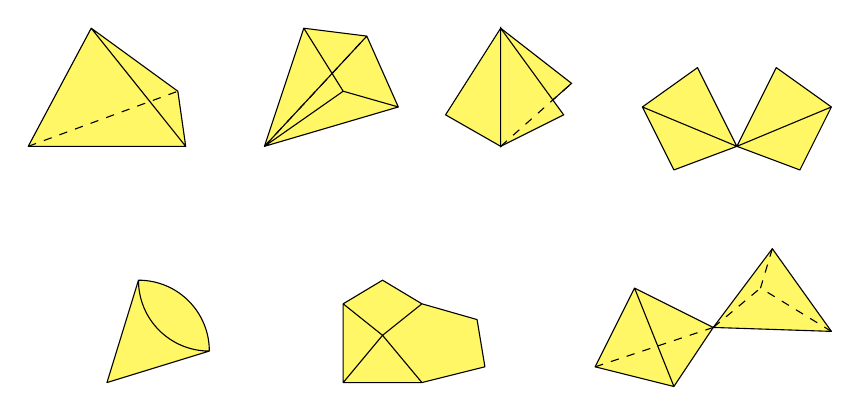
\begin{tikzpicture}[vertexPlain=nolabels, edgeStyle=nolabels, faceStyle=nolabels]
                        % We need to define the drawing style
	
		        % First a tetrahedron
		        \begin{scope}[xshift=0cm]
			    \coordinate (A) at (0,0);
			    \coordinate (B) at (2,0);
		    	    \coordinate (C) at (0.8,1.5);
			    \coordinate (D) at (1.9,0.7);
			
                            \draw[face,edge]
                                (A) -- (B) -- (C) -- cycle
                                (B) -- (C) -- (D) -- cycle;
			    \draw[dashed,edge] (A) -- (D);
		        \end{scope}
		
		        % Second: four triangles in the form of a cone
		        \begin{scope}[xshift=3cm]
			    \coordinate (A) at (0,0);
			    \coordinate (B) at (1.7,0.5);
			    \coordinate (C) at (1.3,1.4);
			    \coordinate (D) at (0.5,1.5);
			    \coordinate (E) at (1,0.7);
			
			    % Take care to draw the faces in the back first
                            \draw[face,edge]
                                (A) -- (B) -- (C) -- cycle
                                (A) -- (C) -- (D) -- cycle
                                (A) -- (B) -- (E) -- cycle
                                (A) -- (E) -- (D) -- cycle;
                            \draw[edge, dashed] (A) -- (C);
		        \end{scope}
		
		        % Three triangles that share an edge
		        \begin{scope}[xshift=6cm]
                                    \coordinate (A) at (0,0);
                            \coordinate (B) at (0,1.5);
                            \coordinate (C) at (-0.7,0.4);
                            \coordinate (D) at (0.8,0.4);
                            \coordinate (E) at (0.9,0.8);
			
                            % draw back face first
                            \filldraw[face] (A) -- (B) -- (E) -- cycle;
                            % Now draw front faces
                            \filldraw[face] (A) -- (B) -- (C) -- cycle;
                            \filldraw[face] (A) -- (B) -- (D) -- cycle;
                            % Draw dashed line
                            \draw[dashed] (A) -- (E);


		        \end{scope}
		
		        % A butterfly of triangles
		        \begin{scope}[xshift=9cm]
                            \def\LUX{-0.8}
\def\LUY{-0.3}
\def\LMX{-1.2}
\def\LMY{0.5}
\def\LOX{-0.5}
\def\LOY{1}
\coordinate (A) at (0,0);
\coordinate (B) at (\LUX,\LUY);
\coordinate (C) at (\LMX,\LMY);
\coordinate (D) at (\LOX,\LOY);
\coordinate (E) at (-\LOX,\LOY);
\coordinate (F) at (-\LMX,\LMY);
\coordinate (G) at (-\LUX,\LUY);
			
\draw[face,edge]
    (A) -- (B) -- (C) -- cycle
    (A) -- (C) -- (D) -- cycle;
\draw[faceSwap, edge]
    (A) -- (E) -- (F) -- cycle
    (A) -- (F) -- (G) -- cycle;

		        \end{scope}
		
		        % An open cone of two triangles
		        \begin{scope}[xshift=1cm, yshift=-3cm]
			    \coordinate (A) at (0,0);
			    \coordinate (B) at (1.3,0.4);
			    \coordinate (C) at (0.4,1.3);
			
                            \draw[face, edge]
                                (A) -- (B) to[bend right=45] (C) -- cycle
                                (A) -- (B) to[bend left=45] (C) -- cycle;
		        \end{scope}
		
		        % A surface from non-triangular shapes
		        \begin{scope}[xshift=4cm, yshift=-3cm]
			    \coordinate (A) at (0,0);
			    \coordinate (B) at (1,0);
			    \coordinate (C) at (0.5,0.6);
			    \coordinate (D) at (0,1);
			    \coordinate (E) at (0.5,1.3);
			    \coordinate (F) at (1,1);
			    \coordinate (G) at (1.7,0.8);
			    \coordinate (H) at (1.8,0.2);
			
                            \draw[face, edge]
                                (A) -- (B) -- (C) -- cycle
                                (A) -- (C) -- (D) -- cycle
                                (D) -- (C) -- (F) -- (E) -- cycle
                                (C) -- (F) -- (G) -- (H) -- (B) -- cycle;
		        \end{scope}

                        % Double tetrahedron
                        \begin{scope}[xshift=8.7cm, yshift=-2.3cm, scale=0.5]
                            % First tetrahedron is ABCD, second one is DEFG
\coordinate (A) at (-3,-1);
\coordinate (B) at (-1,-1.5);
\coordinate (C) at (-2,1);
\coordinate (D) at (0,0);
\coordinate (E) at (3,-0.1);
\coordinate (F) at (1.5,2);
\coordinate (G) at (1.2,1);

\draw[edge, face]
    (A) -- (B) -- (C) -- cycle
    (B) -- (C) -- (D) -- cycle;
\draw[edge, faceSwap] (D) -- (F) -- (E) -- cycle;

\draw[edge, dashed]
    (A) -- (D) (E) -- (G) (D) -- (G) (F) -- (G);

                        \end{scope}
                    \end{tikzpicture}
 

    \end{center}
    \pause
    $\leadsto$ examples of \textbf{polygonal complexes}
\end{frame}

\begin{frame}
    \frametitle{No embedding}
    \pause
    We do not work with embeddings (mostly)
    \begin{itemize}
        \pause
        \item is very hard to compute %TODO example of pentagon flippy?
        \pause
        \item if often unknown for an abstractly constructed surface
        \pause
        \item is different from \textit{intrinsic structure}
        \pause
        \item[$\Rightarrow$] lengths and angles are not important
        \pause
        \item[$\leadsto$] incidence structure is intrinsic
    \end{itemize}
\end{frame}

\begin{frame}[fragile]
    % The option is needed: https://tex.stackexchange.com/questions/119309/arguments-of-tikzset-inside-a-beamer-document
    \frametitle{Incidence structure of a polygonal complex}
    \onslide<2->{
        A \textbf{polygonal complex} consists of
    }
    
    \begin{itemize}
        \item<3-> set of vertices $\mathcal{V}$ \hfill
            \onslide<4->{
                \begin{tikzpicture}
                    \newcommand{\vertexDot}[2]{
                        % xshift, label
                        \coordinate[label={[\vertexColor]right:#2}] (V#2) at (#1,0);
                        \fill[vertex] (V#2) circle (\vSize);
                    }

                    \onslide<4-9>{
                        \vertexDot{0}{2}
                    }
                    \onslide<4-12>{
                        \vertexDot{1}{3}
                        \vertexDot{2}{5}
                    }
                    \onslide<4-14>{
                        \vertexDot{3}{7}
                    }
                    \onslide<4-19>{
                        \vertexDot{4}{11}
                    }
                \end{tikzpicture}
            }
        \item<5-> set of edges $\mathcal{E}$ \hfill
            \onslide<6->{
                {\small
                \begin{tikzpicture}[scale=0.9]
                    \newcommand{\storedEdge}[2]{
                        \coordinate (A#2) at (-0.6+#1*1.5, -0.3);
                        \coordinate (B#2) at (0.6+#1*1.5, 0.3);
                        \draw[edge] (A#2) -- (B#2);
                        \drawEdge{A#2}{B#2}{#2}
                    }

                    \onslide<6-9>{
                        \storedEdge{0}{6}
                    }
                    \onslide<6-12>{
                        \storedEdge{1}{8}
                        \storedEdge{2}{9}
                    }
                    \onslide<6-16>{
                        \storedEdge{3}{10}
                    }
                    \onslide<6-19>{
                        \storedEdge{4}{12}
                        \storedEdge{5}{13}
                    }
                \end{tikzpicture}
                }
            }
        \item<7-> set of faces $\mathcal{F}$ \hfill
            \onslide<8->{
                {\small
                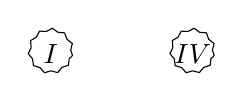
\begin{tikzpicture}[scale=0.9,
                        decoration={snake, amplitude=0.5, segment length=4.5}]
                    \onslide<8-10>{
                        \node at (0,0) {$I$};
                        \draw[decorate] (0,0) circle (0.3);
                    }
                    \onslide<8-18>{
                        \node at (2,0) {$IV$};
                        \draw[decorate] (2,0) circle (0.3);
                    }
                \end{tikzpicture}
                }
            }
        \item<9-> transitive relation \def\brSize{\big}
            $\subset \brSize(\mathcal{V} \times \mathcal{E} \brSize)
            \uplus \brSize(\mathcal{V} \times \mathcal{F} \brSize)
            \uplus \brSize(\mathcal{E} \times \mathcal{F} \brSize)$
    \end{itemize}
    % Draw the pictures
    \onslide<10->{
        \begin{tikzpicture}[vertexNode/.style={circle, draw=\vertexColor}, node distance=0.5]

            % Edge nodes
            % name, position, text, minimal slide
            \newcommand{\edgeNode}[4]{
                \onslide<#4->{
                    \node[edgeBackground] (#1) [#2] {#3};
                }
                \onslide<-#4-1>{
                    \node (#1) [#2] {};
                }
            }
            \node[edgeBackground] (E6) { 6 };
            \edgeNode{E8}{right=of E6}{8}{13}
            \edgeNode{E9}{right=of E8}{9}{13}
            \edgeNode{E10}{right=of E9}{10}{17}
            \edgeNode{E12}{right=of E10}{12}{20}
            \edgeNode{E13}{right=of E12}{13}{20}

            % Face nodes
            % name, position, text, minimal slide
            \newcommand{\faceNode}[4]{
                \onslide<#4->{
                    \node (#1) [#2] {#3};
                }
                \onslide<-#4-1>{
                    \node (#1) [#2] {};
                }
            }
            \faceNode{F1}{above=of E8}{$I$}{11}

            \onslide<11->{
                \draw (F1) -- (E6);
            }
            \onslide<13->{
                \draw (E8) -- (F1) -- (E9);
            }

            \node (Help) at ($(E10)!0.5!(E12)$) {};
            \faceNode{F4}{above=of Help}{$IV$}{19}
            \onslide<19->{
                \draw (E9) -- (F4) -- (E10);
            }
            \onslide<20->{
                \draw (E12) -- (F4) -- (E13);
            }

            % Vertex nodes
            % name, position, text, minimal slide
            \newcommand{\vertexNode}[4]{
                \onslide<#4->{
                    \node[vertexNode] (#1) [#2] {#3};
                }
                \onslide<-#4-1>{
                    \node (#1) [#2] {};
                }
            }
            \vertexNode{V7}{below=of Help}{7}{15}
            \onslide<17->{
                \draw (E10) -- (V7);
            }
            \onslide<20->{
                \draw (E13) -- (V7);
            }
            \vertexNode{V11}{right=of V7}{11}{20}
            \onslide<20->{
                \draw (E13) -- (V11) -- (E12);
            }
            \vertexNode{V5}{left=of V7}{5}{14}
            \onslide<13->{
                \draw (E8) -- (V5) -- (E9);
            }
            \onslide<20->{
                \draw (E12) -- (V5);
            }

            \vertexNode{V4}{left=of V5}{3}{14}
            \onslide<14->{
                \draw (E6) -- (V4) -- (E9);
            }
            \onslide<17->{
                \draw (E10) -- (V4);
            }
            \vertexNode{V2}{left=of V3}{2}{10}
            \onslide<10->{
                \draw (E6) -- (V2);
            }
            \onslide<13->{
                \draw (E8) -- (V2);
            }

            \begin{scope}[xshift=7cm, yshift=-0.6cm, scale=0.7]
                %       P3 ------------ P4
                %      / |       10     | 
                %    6/  |              |
                %    /   |              |
                %  P1  I |9      IV     |13
                %    \   |              |
                %    8\  |              |
                %      \ |        12    |
                %       P2 ------------ P5

                % name, position, label, label position, minimal slide
                \newcommand{\vCoord}[5]{
                    \onslide<#5->{
                        \coordinate[label={[vertex]#4:#3}] (#1) at #2;
                    }
                    \onslide<-#5-1>{
                        \coordinate (#1) at #2;
                    }
                }
                \vCoord{P1}{(0,0.5)}{2}{left}{10}
                \vCoord{P2}{(2,-1)}{5}{below}{14}
                \vCoord{P3}{(2,2)}{3}{above}{14}
                \vCoord{P4}{(5,2)}{7}{above}{15}
                \vCoord{P5}{(5,-1)}{11}{below}{20}

                % Draw first face
                \onslide<13->{
                    \filldraw[face] (P1) -- (P2) -- (P3) -- cycle;
                    \node at ($1/3*(P1)+1/3*(P2)+1/3*(P3)$) {I};
                }
                \onslide<11-12>{
                    \fill[\faceColor] (P1) -- (P2) -- (P3) -- cycle;
                    \node at ($1/3*(P1)+1/3*(P2)+1/3*(P3)$) {I};
                }
                \onslide<10-12>{
                    \draw[\edgeColor] (P1) -- (P3);
                }

                % Draw the second face
                \onslide<20->{           
                    \filldraw[face] (P2) -- (P3) -- (P4) -- (P5) -- cycle;
                    \node at ($1/4*(P2)+1/4*(P3)+1/4*(P4)+1/4*(P5)$) {IV};
                }
                \onslide<19->{
                    \fill[\faceColor] (P2) -- (P3) -- (P4) -- (P5) -- cycle;
                    \node at ($1/4*(P2)+1/4*(P3)+1/4*(P4)+1/4*(P5)$) {IV};
                }
                \onslide<17-19>{
                    \draw[\edgeColor] (P3) -- (P4);
                }
        

                % Draw the edges
                \onslide<10->{
                    \drawEdge{P1}{P3}{6}
                }
                \onslide<13->{
                    \drawEdge{P1}{P2}{8}
                    \drawEdge{P2}{P3}{9}
                }
                \onslide<17->{
                    \drawEdge{P3}{P4}{10}
                }
                \onslide<20->{
                    \drawEdge{P4}{P5}{13}
                    \drawEdge{P5}{P2}{12}
                }

                % Draw the concrete points
                \onslide<10->{
                    \fill[vertex] (P1) circle (\vSize);
                }
                \onslide<13->{
                    \fill[vertex] (P2) circle (\vSize);
                    \fill[vertex] (P3) circle (\vSize);
                }
                \onslide<15->{
                    \fill[vertex] (P4) circle (\vSize);
                }
                \onslide<20->{
                    \fill[vertex] (P5) circle (\vSize);
                }
            \end{scope}
        \end{tikzpicture}
    }
    \begin{enumerate}
        \item<12-> Every face is a polygon
        \item<16-> Every vertex lies in an edge \onslide<18->{and every edge lies in a face}
    \end{enumerate}
\end{frame}


\begin{frame}{Polygonal complexes}
    A \textbf{polygonal complex} is
    \pause
    a two--dimensional incidence structure of vertices, edges and faces, such that:
    \begin{enumerate}
        \pause
        \item Every edge has exactly two vertices.
            \begin{tikzpicture}
                \coordinate[label={[vertex]left:2}] (A) at (0,0);
                \coordinate[label={[vertex]right:3}] (B) at (3,0);

                \draw (A) -- (B);
                \drawEdge{A}{B}{6}

                \foreach \p in {A,B}
                    \fill[vertex] (\p) circle (\vSize);
            \end{tikzpicture}
        
        \pause
        \item Every face is a polygon.
            \pause
            \begin{center}
                \begin{tikzpicture}
                % We will do a pentagon
                \def\r{1.5}
                \coordinate [label={[vertex]right:$v_1$}] (P1) at (306:\r);
                \coordinate [label={[vertex]right:$v_2$}] (P2) at (18:\r);
                \coordinate [label={[vertex]above:$v_3$}] (P3) at (90:\r);
                \coordinate [label={[vertex]left:$v_4$}] (P4) at (162:\r);
                \coordinate [label={[vertex]left:$v_5$}] (P5) at (234:\r);

                \filldraw[face] (P1) -- (P2) -- (P3) -- (P4) -- (P5) -- cycle;

                \foreach \p in {P1,P2,P3,P4,P5}
                    \fill[vertex] (\p) circle (\vSize);

                \drawEdge{P1}{P2}{$e_1$}
                \drawEdge{P2}{P3}{$e_2$}
                \drawEdge{P3}{P4}{$e_3$}
                \drawEdge{P4}{P5}{$e_4$}
                \drawEdge{P5}{P1}{$e_5$}

                \node[scale=2] at (0,0) {$\circlearrowleft$};
            \end{tikzpicture}
            \end{center}
        \pause
        \item Every vertex lies in an edge
        \pause
        \item Every edge lies in a face
    \end{enumerate}
\end{frame}


\begin{frame}{Isomorphism testing}
    \pause
    Incidence geometry allows ``easy" isomorphism testing.
    \pause
    Incidence structure can be interpreted as a coloured graph:
    \pause
        \begin{center}
        \begin{tikzpicture}[vertexNode/.style={circle,
            fill=magenta!50!white}, node distance=0.5]
            % Edge nodes
            \node[edgeBackground] (E6) {6};
            \node[edgeBackground] (E8) [right=of E6] {8};
            \node[edgeBackground] (E9) [right=of E8] {9};
            \node[edgeBackground] (E10) [right=of E9] {10};
            \node[edgeBackground] (E12) [right=of E10] {12};
            \node[edgeBackground] (E13) [right=of E12] {13};

            % Face nodes
            \node[fill=yellow] (F1) [above=of E8] {$I$}
                edge (E6) edge (E8) edge (E9);
            \node (Help) at ($(E10)!0.5!(E12)$) {};
            \node[fill=yellow] (F4) [above=of Help] {$IV$}
                edge (E9) edge (E10) edge (E12) edge (E13);

            % Vertex nodes
            \node[vertexNode] (V7) [below=of Help] {7}
                edge (E10) edge (E13);
            \node[vertexNode] (V11) [right=of V7] {11}
                edge (E13) edge (E12);
            \node[vertexNode] (V5) [left=of V7] {5}
                edge (E8) edge (E9) edge (E12);
            \node[vertexNode] (V3) [left=of V5] {3}
                edge (E6) edge (E9) edge (E10);
            \node[vertexNode] (V2) [left=of V3] {2}
                edge (E6) edge (E8);
        \end{tikzpicture}
        \end{center}
    \pause
    $\leadsto$ reduce to graph isomorphism problem

    \pause
    Solved by NautyTracesInterface (by Gutsche, Niemeyer, Schweitzer)
\end{frame}


\begin{frame}{General properties}
    \pause
    Some properties can be computed for all polygonal complexes:
    \pause
    \begin{itemize}
        \item Connectivity
        \pause
        \item Euler--Characteristic
    \end{itemize}
    \pause
    \textit{Orientability} is \textbf{not} one of them.
    \pause
    Counterexample:
        \begin{center}
            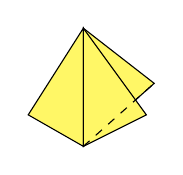
\begin{tikzpicture}
                \coordinate (A) at (0,0);
                \coordinate (B) at (0,1.5);
                \coordinate (C) at (-0.7,0.4);
                \coordinate (D) at (0.8,0.4);
                \coordinate (E) at (0.9,0.8);
                			
                % draw back face first
                \filldraw[face] (A) -- (B) -- (E) -- cycle;
                % Now draw front faces
                \filldraw[face] (A) -- (B) -- (C) -- cycle;
                \filldraw[face] (A) -- (B) -- (D) -- cycle;
                % Draw dashed line
                \draw[dashed] (A) -- (E);
	    \end{tikzpicture}
        \end{center}
    \pause
    $\Rightarrow$ every edge lies in at most two faces (for well--definedness)
    
    \pause
    $\leadsto$ \textbf{ramified polygonal surfaces}
\end{frame}


\begin{frame}{Why ramified?}
    \pause
    Typical example of ramified polygonal surface:
    \pause
    \begin{center}
        \begin{tikzpicture}
                % First tetrahedron is ABCD, second one is DEFG
                \coordinate (A) at (-3,-1);
                \coordinate (B) at (-1,-1.5);
                \coordinate (C) at (-2,1);
                \coordinate (D) at (0,0);
                \coordinate (E) at (3,-0.1);
                \coordinate (F) at (1.5,2);
                \coordinate (G) at (1.2,1);
                
                \filldraw[face] (A) -- (B) -- (C) -- cycle;
                \filldraw[face] (B) -- (C) -- (D) -- cycle;
                \filldraw[faceAlt] (D) -- (F) -- (E) -- cycle;
                
                \draw[dashed] (A) -- (D);
                \draw[dashed] (E) -- (G);
                \draw[dashed] (D) -- (G);
                \draw[dashed] (F) -- (G);
        \end{tikzpicture}
    \end{center}
    \pause
    $\Rightarrow$ It is not a surface -- there is a \textit{ramification} at 
        the central vertex
    
    \pause
    A \textbf{polygonal surface} does not have these ramifications.
\end{frame}



            
%%%%%%%%%%%%%%%%%%%%%%%%%%%%%%%%%%%%%%%%%%%%%%%%%%%%%%%%%%
%%
%%              Second section
%%
\section{Edge colouring and group properties}
\newcommand{\colA}{blue}
\newcommand{\colB}{red}
\newcommand{\colC}{green!80!black}
\newcommand{\width}{very thick}
\frame{\tableofcontents[currentsection]}


\begin{frame}{Embedding question}
    \pause
    Given: A polygonal complex
    \begin{itemize}
        \pause
        \item Can it be embedded?
        \pause
        \item In how many ways?
    \end{itemize}
    \pause
    Simplifications:
    \begin{enumerate}
        \pause
        \item Only polygonal surfaces (surface that is build from polygons)
        \pause
        \item All polygons are triangles (\textbf{simplicial surfaces})
        \pause
        \item All triangles are isometric
    \end{enumerate}
    \pause
    $\leadsto$ Edge--colouring encodes different lengths
            \begin{center}
                %       F
                %    C     E 
                % A     B    D
                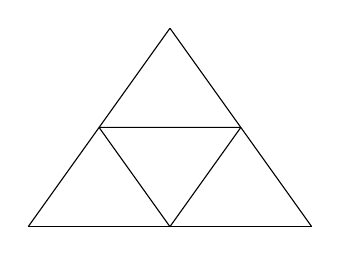
\begin{tikzpicture}[scale=0.9]
                    \coordinate (A) at (0,0);
                    \coordinate (B) at (2,0);
                    \coordinate (C) at (1,1.4);
                    \coordinate (D) at ($2*(B)$);
                    \coordinate (E) at ($(B)+(C)$);
                    \coordinate (F) at ($2*(C)$);

                    \draw[\colA, \width] (A) -- (B) -- (D);
                    \draw[\colA, \width] (C) -- (E);
                    \draw[\colB, \width] (B) -- (C);
                    \draw[\colB, \width] (D) -- (E) -- (F);
                    \draw[\colC, \width] (A) -- (C) -- (F);
                    \draw[\colC, \width] (B) -- (E);
                \end{tikzpicture}
            \end{center}
\end{frame}


\begin{frame}{How do faces fit together?}
    \onslide<2->{
        Consider a face of the surface \onslide<4->{and a neighbouring face}
    }

    \onslide<6->{
        The neighbour can be coloured in two ways:
    }
    \onslide<1->{
        \begin{center}
        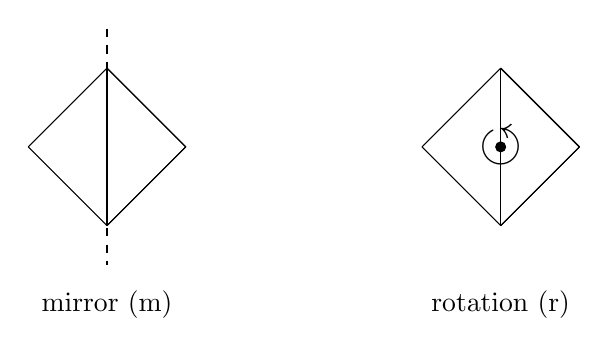
\begin{tikzpicture}
            % Numbers to determine drawing
            \def\x{1}
            \def\y{1}

            %      B
            %    / | \
            %   A  |  D
            %    \ | /
            %      C
            
            % First pair
            \begin{scope}
                \coordinate (A) at (0,0);
                \coordinate (B) at (\x,\y);
                \coordinate (C) at (\x,-\y);
                \coordinate (D) at (2*\x,0);

                \onslide<3->{
                    \draw[\colA,\width] (A) -- (B);
                    \draw[\colB,\width] (A) -- (C);
                    \draw[\colC,\width] (B) -- (C);
                }
                \onslide<5->{
                    \draw (B) -- (D) -- (C);
                }
                \onslide<7->{
                    \draw[\colA,\width] (B) -- (D);
                    \draw[\colB,\width] (C) -- (D);
                }
                \onslide<9->{
                    % Draw mirror line
                    \draw[dashed, thick] (\x,1.5*\y) -- (\x,-1.5*\y);
                    \node at (\x,-2*\y) {mirror (m)};
                }
            \end{scope}

            % Second pair
            \begin{scope}[xshift=5cm]
                \coordinate (A) at (0,0);
                \coordinate (B) at (\x,\y);
                \coordinate (C) at (\x,-\y);
                \coordinate (D) at (2*\x,0);

                \onslide<6->{
                    \draw[\colA,\width] (A) -- (B);
                    \draw[\colB,\width] (A) -- (C);
                    \draw[\colC,\width] (B) -- (C);
                    \draw (B) -- (D) -- (C);
                }
                \onslide<8->{
                    \draw[\colB,\width] (B) -- (D);
                    \draw[\colA,\width] (C) -- (D);
                }
                \onslide<10->{
                    % Draw rotation center and circle
                    \fill[black] (\x,0) circle (2pt);
                    \node[scale=2] at (\x,0) {$\circlearrowleft$};
                    \node at (\x,-2*\y) {rotation (r)};
                }
            \end{scope}
        \end{tikzpicture}
        \end{center}
    }
    \onslide<11->{
        This gives an \textbf{mr--assignment} for the edges.
    }
\end{frame}

%%%%%%%%%%%%%%%%%%%%%%%%%%%%%%%%%%%%%%%%%%%%%%%%%%%%%%%%%%%%%%
%%
%%    Third section
%%
\section{Abstract folding}
\frame{\tableofcontents[currentsection]}


\end{document}
